\chapter{Analýza}
\label{chapter:analyza}
Hlavním cílem teto bakalářské práce je implementovat návrh backendu podle návrhu a fragmentu implementace, které byly udělány v rámci předmětů BI-SP1 a BI-SP2 bakalářského studia vyučovaných na FIT ČVUT v akademickém roce 2018/2019 a 2019/2020. Tato kapitola se zabývá analýzou výsledků zmíněných předmětu. Autor práce je zároveň i absolventem těchto předmětů, kde pracoval v týmu na analýze požadavku zákazníka a pak pracoval jako backend vývojář a vedoucí backendového týmu.

Pro jasné zajištěni verze aplikace, která bude předmětem analýzy teto kapitoly, uvádím datům ukončení práce na projektu v rámci předmětu BI-SP2 - 25. února 2020. Také pro možnost pohodlně vyhledat konkretní verze uvádím poslední 
\textit{commit}\footnote{252b0288dbfe9942446b78fd452c0edce810a370} udělaný v rámci tohoto předmětu.

% Tato kapitola se zabývá popisem současného stavu aplikace, který je výsledkem zmíněných předmětů.

% Hlavním cílem teto bakalářské práce je implementovat návrh backendu podle návrhu a fragmentu implementace, které byly rozpracovány v rámci předmětů BI-SP1 BI-SP2 bakalářského studia vyučovaných na FIT ČVUT. Dalším cílem teto práci je navrhnou vhodné úpravy za účelem dosažení kvalitnějšího výsledku a splnění požadavku frontedové častí aplikace. Autor teto práci absolvoval zmíněné předměty, proto pro zajištění rozdilu v 

    \section{Analýza současného návrhu} \label{analyza:analyza navrhu}
    
     \subsection{Předmět BI-SP1}\label{analyza:navrh:sp1}
        V rámci předměty BI-SP1 pracovalo sedm lidí včetně autora teto práci. Tým měl za úkol analýz požadavku zákazníka a návrh implementaci aplikace. Aplikace se skládá ze dvou částí. Serverového backendu, který je předmětem teto bakalářské práci a frontendové častí aplikace, kterou současně v rámci bakalářské prací implementuje kolega - Martin Beran. Frontendová část aplikace je Android aplikací. Backendová část je serverovým backendém, který má poskytovat REST\footnote{Representational State Transfer} API pro Android aplikaci.
    
        Během semestru tým provedl kompletní analýzu požadavku zákazníka. Především, tým navrhl scénáře použiti aplikace:
        \begin{itemize}
	        \item Přihlašování/Registrace;
	        \item Přihlašování/Registrace do rodiny;
	        \item Role v aplikace a jejich vytváření;
	        \item Nastavení pečovatelský dnů;
	        \item Kalendář;
	        \item Kniha potřeb dítěte;
	        \item Uchování účtenek;
	        \item Správa alimentů.
        \end{itemize}
        Potom byly navrženy Use Case Diagram a Activity Diagramy, podle kterých byly navrženy Wireframy a Doménový model. 
    
    \subsection{Předmět BI-SP2}\label{analyza:navrh:sp2}
        Cílem předmětu BI-SP2 byla implementace návrhu předmětu BI-SP2. Autor teto práce pracoval v backendovém týmu a zároveň vystupoval v roli vedoucího backendového týmu.
        
        Pro vývoj backendové častí aplikace byl zvolen jazyk Kotlin, zmíněný v sekci \ref{resere:kotlin}, a framework Spring, zmíněný v sekci \ref{resere:j2ee}. Jako {buildovací system}\footnote{nástroj pro automatizaci sestavování programu} byl zvoleny nástroj Gradle. Podrobnnějí výsledky předmětu BI-SP2 probrány v sekce \ref{analyza:soucasnaImplementace}.
        
    
    \subsection{Doménový model}\label{analyza:navrh:DomainModel}
        Hlavním zdrojem informace o výsledném návrhu serveru je Doménový model. Kompletní Doménový model se nachází v příloze \ref{dodatek:DomainModel}. Zelenou barvou jsou označeny třídy, které už jsou implementovány. žlutou barvou jsou označeny třídy, které ještě nejsou implementovány. Také, jsou třídy označeny zároveň žlutou a zelenou barvou, což znamená, že třída je implementována jenom částečně. Taková situace se mohla nastat v případe, že implementace vyžadovala implementace jiné třídy, která ještě neexistovala. Tento Doménový model má určité nedostatky podle požadavku frontedové části aplikace. Jako příklad takových nedostatku je možné uvést zbytečně komplikovaný návrh Intervalů (viz. obrázek \ref{image:Interval1}), který byl od začátku předělán.

    \subsection{Registrace a přihlášeni do rodiny}
        Aplikace je navržena tak, že první uživatel, který má vytvořit svůj účet je jeden z rodičů. Pro registraci člověk potřebuje řadu povinných údajů:
        \begin{itemize}
	        \item \textit{name} - zvolené jméno se stává jeho implicitním jménem v systému
	        \item \textit{surname} - zvolené příjmení se stává jeho implicitním příjmením v systému
	        \item \textit{email} - zvolený email je identifikátorem uživatele v rámci systému
	        \item \textit{password} - heslo pro autorizaci v systému
        \end{itemize}
        Na základe těchto údajů se vytváří unikátní uživatel v rámci systému. V tomto stavu člověk není přihlášeny do žádné rodiny a nemá žádnou roli. Podrobněji role budou popsané v sekci \ref{analyza:bezpecnost:role}. \textit{User} také může mít implicitní obrázek profilu (viz. obrázek \ref{image:User-Image1}).
        \begin{figure}\centering
	        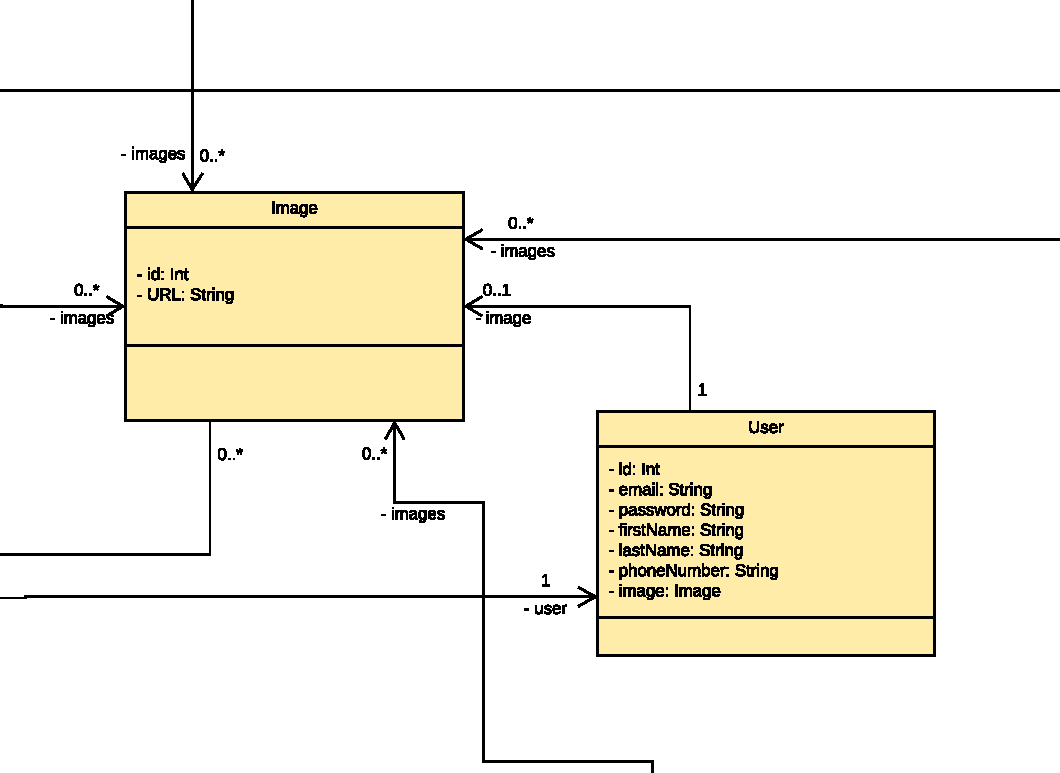
\includegraphics[width=0.5\textwidth]{pdfs/User-Image1}
	        \caption[Návrh User-Image]{Vztah mezi třídami \textit{User} a \textit{Image} podle Doménovém modelu z předmětu BI-SP2}\label{image:User-Image1}
        \end{figure}
        
        Potom uživatel má možnost vytvořit rodinu nebo přihlásit se do již existující rodiny. Pro vytvoření nové rodiny, uživatel potřebuje zadat jméno rodiny a přidat členy rodiny. Autor teto rodiny automaticky se stává jedním s rodičů teto rodiny. jinou možností je přihlásit se do rodiny, která již existuje. Podmínkou k tomu je existování pozvání do některé existující rodiny. V takovém případě uživatel už nemá možnost zvolit role v rámci rodiny. Role má být nastavena uživatelem, který vytvořil toto pozvání.

    \subsection{Kalendář}    
        Kalendář je hlavním zdrojem informaci pro celou rodinu, který společný pro všechny uživatele. Na něm jsou zobrazené zvýrazněné různými barvami pečovatelské dny obou rodičů a důležité události, které mohou být jednorázové nebo pravidelné. 
        
        Kromě dlouhodobých nastavení pečovatelských dnu, kalendář může zobrazovat i jednorázové změny, které mohou vidět všechny členy rodiny. Takový postup pomáhá rodině eliminovat situace, kdy několik členu rodiny najednou myslí, že je v konkretní den dítě v jejích péči nebo několik členu rodiny najednou říkají, že není to jejích den.  
    \subsection{Alimenty}    
        Aplikace řeší i finanční problémy. Hlavní problémem jsou alimenty, které má pravidelně uhrazovat jeden z rodičů. Tento proces byl rozdělen do dvou častí. První častí je nastavení dlouhodobých pravidel (viz. obrázek \ref{image:AlimonySettings1}) pro splacení alimentů. Druhou častí jsou samotné alimenty (viz. obrázek \ref{image:Alimony1}), které se generuje na základě dlouhodobých nastavení. Jedna rodina může mít zároveň několik nastavení v případě, že jedna rodina má několik dětí nebo chce rozdělit alimenty do logický částí.
        \begin{figure}\centering
	        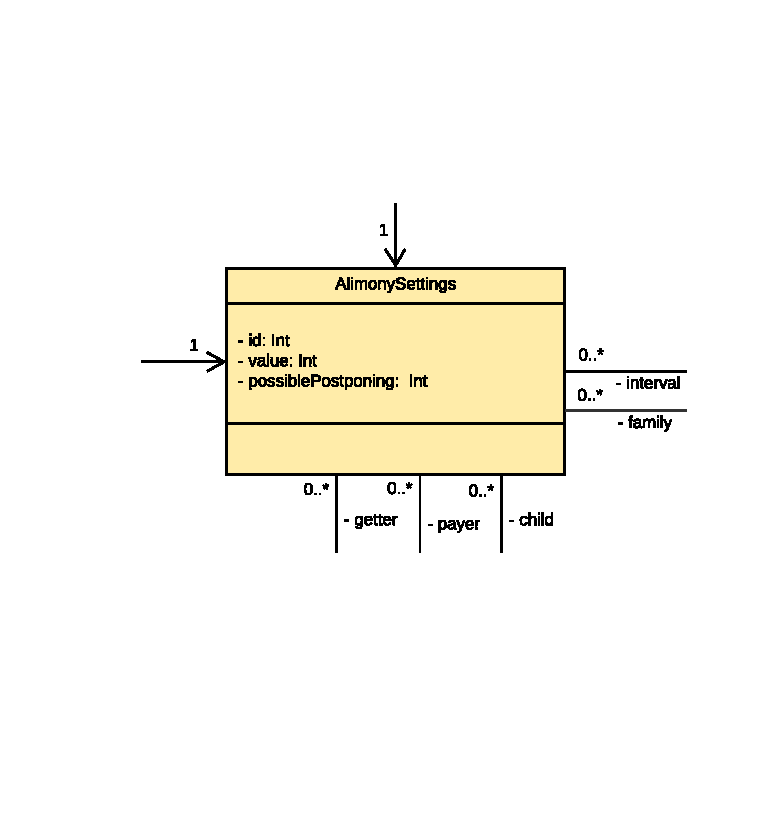
\includegraphics[width=0.5\textwidth]{pdfs/AlimonySettings1}
	        \caption[Návrh AlimonySettings]{Návrh třídy \textit{AlimonySettings} podle Doménovém modelu z předmětu BI-SP2}\label{image:AlimonySettings1}
        \end{figure}
        \begin{figure}\centering
	        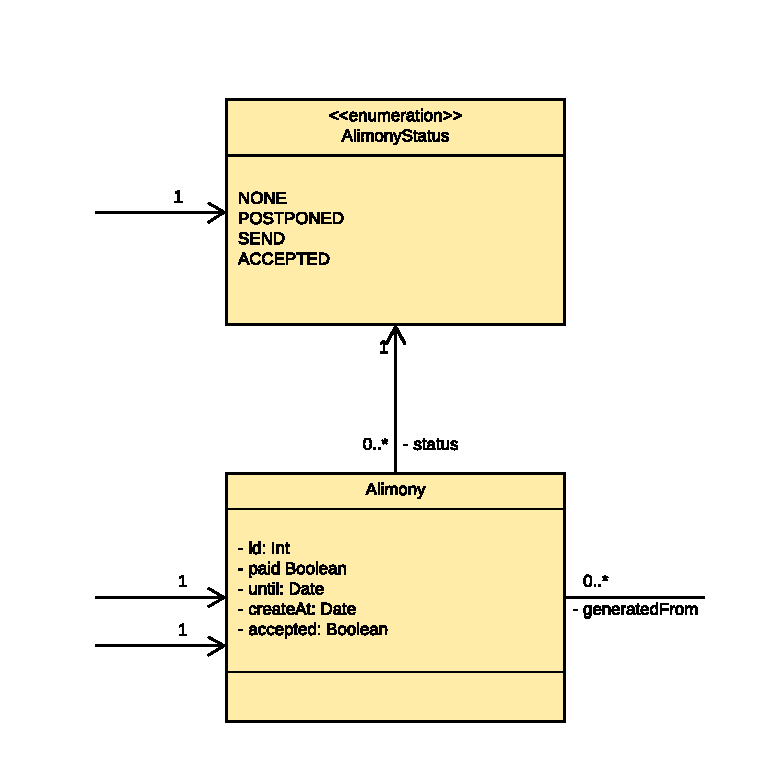
\includegraphics[width=0.5\textwidth]{pdfs/Alimony1}
	        \caption[Návrh Alimony]{Návrh třídy \textit{Alimony} podle Doménovém modelu z předmětu BI-SP2}\label{image:Alimony1}
        \end{figure}
    \subsection{Kniha potřeb dítěte}
    
        Jedním s populárních problému, který vzniká v procesu rozvodu, je nakupování příliš drahých věci o kterých nevědí ostatní členy rodiny. Jako příklad je možné uvést nakupování bot pro dítěte. Jeden s rodičů může chtít "koupit lásku dítěte" a koupit několikrát dražší boty než dítěte opravdu potřebuje. Kniha potřeb dítěte (viz. obrázek \ref{image:Need1}) je zaměřena na překonání takových situací.
        \begin{figure}\centering
	        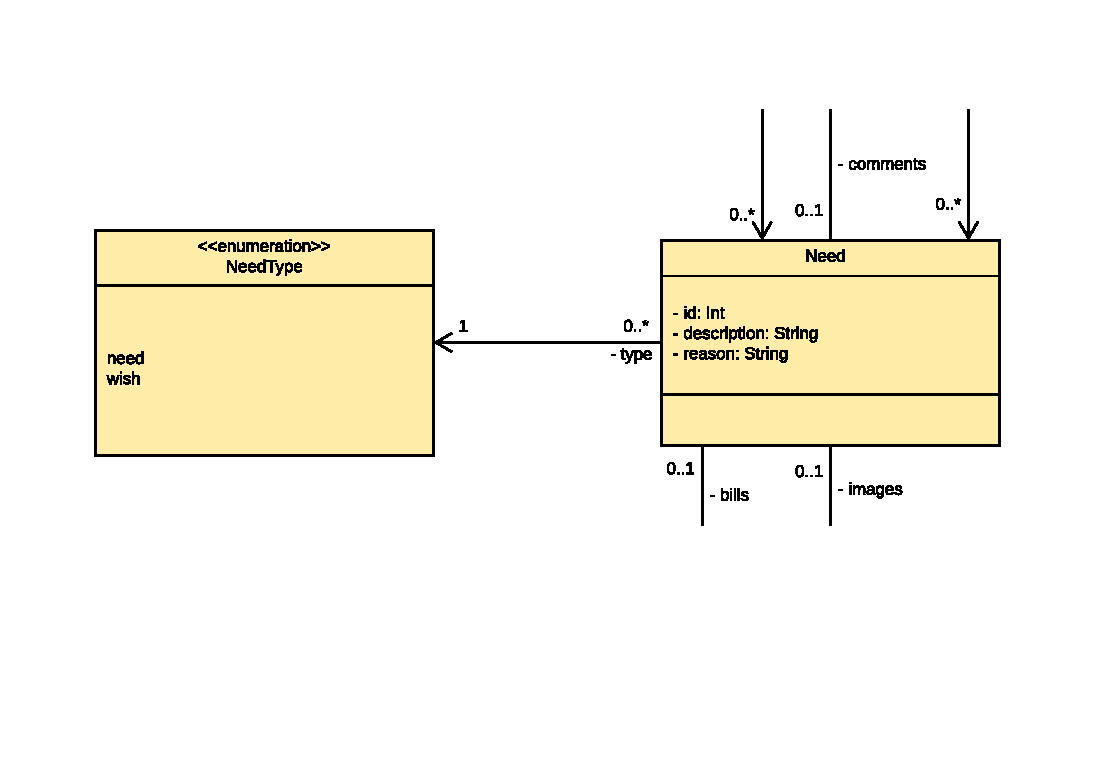
\includegraphics[width=0.5\textwidth]{pdfs/Need1}
	        \caption[Návrh Need]{Návrh třídy \textit{Need} podle Doménovém modelu z předmětu BI-SP2}\label{image:Need1}
        \end{figure}
        
        Potřeba může být typu \textit{need} a \textit{wish}. Podle současného návrhu je rozdíl mezi typy pouze pro informační účely. Každé instance \textit{Need} patři instance \textit{NeedPermission} (viz. obrázek \ref{image:NeedPermissions1}), která definuje přístupová práva pro jednotlivého člena rodiny. V případě, že uživatel nemá žádné z přístupových práv, uživatel nemá ve svém seznamu potřeb dítěte tento záznam.
        \begin{figure}\centering
	        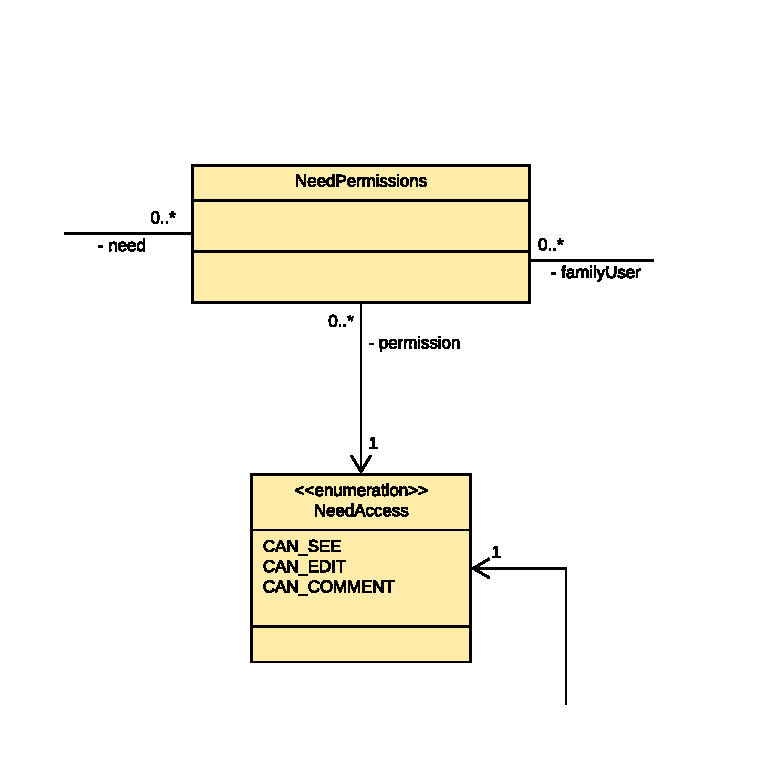
\includegraphics[width=0.5\textwidth]{pdfs/NeedPermissions1}
	        \caption[Návrh NeedPermissions]{Návrh třídy \textit{NeedPermissions} podle Doménovém modelu z předmětu BI-SP2}\label{image:NeedPermissions1}
        \end{figure}
       
       Potřeba má v sobě následující informace:
        \begin{itemize}
            \item \textit{description} - popis potřeby
            \item \textit{reason} - příčina proč dítě tohle potřebuje
            \item \textit{images} - obrázky věcí, kterou dítě potřebuje
            \item \textit{bills} - účtenky v případě, že někdo z rodičů splnil potřebu
            \item \textit{comments} - komentáře členu rodiny včetně dítěte
        \end{itemize}
     
    \section{Analýza současné implementace}\label{analyza:soucasnaImplementace}
        Projekt má ve složce \textit{main}\footnote{bi-springboot/src/main} 69 souborů a 845 řádek kódů. Implementace částečné pokrývá Doménový model zmíněný v sekci. \ref{analyza:navrh:DomainModel}.
        
        Seznam implementovaných entit:
        \begin{itemize}
            \item \textit{AlimonyStatus}
            \item \textit{Bill}
            \item \textit{CalendarEvent}
            \item \textit{OneTimeEvent}
            \item \textit{Comment}
            \item \textit{FamilyMember} - částečně
            \item \textit{History}
            \item \textit{IntervalType}
            \item \textit{NWeekInterval}
            \item \textit{WeekInterval}
            \item \textit{NeedAccess}
            \item \textit{NeedType}
            \item \textit{NeedType}
            \item \textit{AbstractPermissions}
            \item \textit{Permissions}
            \item \textit{RequestStatus}
            \item \textit{User}
        \end{itemize}
        
        Bylo provedeno nastavení frameworku Swagger\ref{resere:dokumentace} pro dokumentace API (viz. obrázek \ref{code:swagger-configuration}). Podrobněji framework Swagger byl popsán v sekci \ref{resere:dokumentace}.
        \begin{figure}
        \begin{minted}{java}
        @Configuration
        @EnableSwagger2
        class SwaggerConfig {
        @Bean
        fun api(): Docket {
            return Docket(DocumentationType.SWAGGER_2)
                .select()
                .apis(RequestHandlerSelectors.any())
                .paths(PathSelectors.any())
                .build()
            }
        }
        \end{minted}
        \caption{Ukázka nastavení frameworku Swagger} 
        \label{code:swagger-configuration}
        \end{figure}
        
        Byl přidány \textit{Controller} pro testování, zda aplikace běží. \textit{Controller} je namapován na \textquote{/}. Také, byl přidaná třída, která obsahuje nápovědy pro ostatní \textit{Controllery} ohledně zachycování chyb. Tato třída byla zavedena za účelem poskytování uživateli jenom korektně formátovanou informaci  a filtrování zbytečné informace pro koncového uživatele (viz. tabulka \ref{tab:excpetion-handler1}). 
        \begin{table}\centering
	    \caption[Exception handler]{Ukázka \textit{Exception handler} podle návrhu BI-SP2}\label{tab:excpetion-handler1}
	        \begin{tabular}{|l|l|c|c|}\hline
		        Typ chyby		& HTTP status		& zprava	& URL	\tabularnewline \hline \hline
		        \textit{IllegalAccessException}	& 401	& původní zprava chyby		& původní cesta     \tabularnewline \hline
		        \textit{IllegalArgumentException}	& 400	& původní zprava chyby		& původní cesta     \tabularnewline \hline
		        \textit{NullPointerException}	& 500	& původní zprava chyby		& původní cesta     \tabularnewline \hline
		        \textit{NoSuchElementException}	& 404	& nic		& nic     \tabularnewline \hline
	        \end{tabular}
        \end{table}
    
    \section{Analýza požadavku frontendu}
        % Po dobu práce backendového týmu v ramci předmětu, frontendový tým pracoval na implementaci Android aplikace. 
    
    \section{Analýza konkurence}
        Tento návrhnjfgndd
% \section{Analýza testování}

    \section{Analýza bezpečnosti}
    
        \subsection{Role}\label{analyza:bezpecnost:role}
    
    % Aplikace je navržená tak, že první věc, kterou uživatel udělat, je registrace. Uživatel potřebuje zvolit jméno, příjmení, email a heslo. Na základě těchto údajů se vytváří účet uživatele. V Doménovém modelu tato třída se jmenuje \textit{User}. V tento okamžik uživatel má role \textit{USER}, která mu nadává možnost udělat jenom omezený počet věcí.  
        Každý uživatel po přihlášeni do rodiny má svou vlastní roli (viz. obrázek \ref{image:Role1}), podle které mohou lišit jeho přístupová práva. 
        \begin{figure}\centering
	        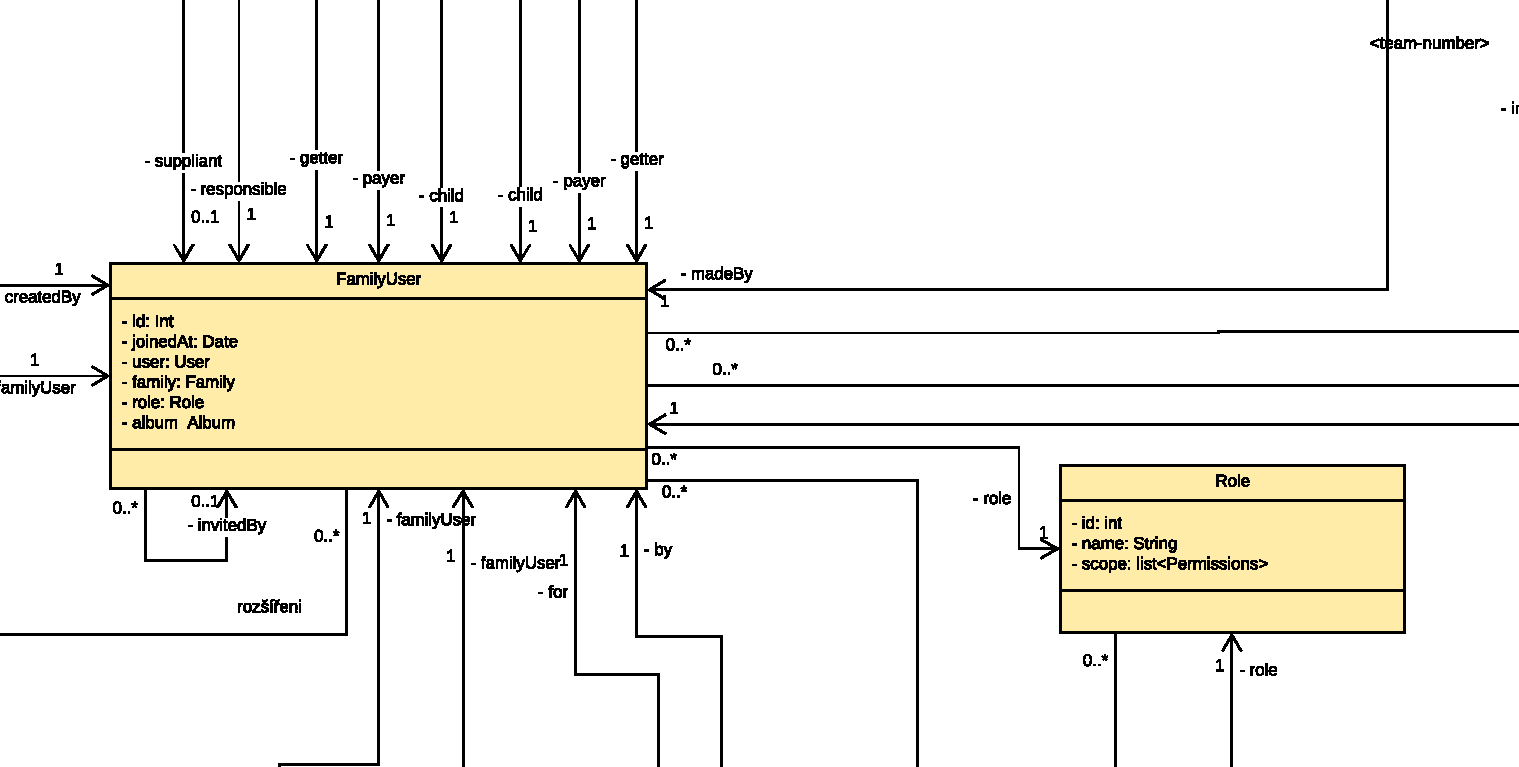
\includegraphics[width=0.7\textwidth]{pdfs/Role1}
	        \caption[Návrh \textit{Role}]{Návrh třídy \textit{Role} podle Doménovém modelu z předmětu BI-SP2}\label{image:Role1}
        \end{figure}
    
        \subsection{Autorizace}
            Bezpečnost serveru je možné rozdělit do dvou častí. 
            Návrh bezpečné aplikace nebyl cílem předmětu zmíněných v sekcích \ref{analyza:navrh:sp1} a \ref{analyza:navrh:sp2}.